\section{Experiments}\label{sec:testing}
In this section we are going to perform a number of experiments on our 456 GB dataset of two million matches. Firstly we are going to perform some initial experiments on a single computer, to get an idea of the strength of features in \Cref{sec:initialtest}. In \Cref{sec:clustertest}, we will present the experiments that have been running on the cluster. Lastly in \Cref{sub:knowledge} we present a list of the knowledge which can be extracted from our results. All following experiments will be performed using a split of $\frac{2}{3}$ for training set and $\frac{1}{3}$ for testing set. 

\subsection{Initial experimentation}\label{sec:initialtest}
In this section we will present experiments which have been run on a smaller dataset, to get a quick overview of the strength of features. 
These experiments are used to find the settings, with which the cluster should be run when the final cluster experiments will be performed. 

\subsubsection{Best machine learning technique}
Many different machine learning algorithms exists for learning a classifier. In this experiment, we test eight different classifiers provided by Weka to see which one gives the best result for our particular problem~\cite{weka}. 
The tested classifiers are naive bayes, hidden naive bayes, logistic regression, neural network, support vector machine (C-SVM), adaboost(using decision stump), Hoeffding tree, and decision stump. 
All the different methods are run with multiple parameter settings to find the configuration that yields the best result. 
Note that naive bayes, hidden naive bayes and decision stump takes no parameters. 
For logistic regression, different values of the L2-regularisation parameter has been tested. 
For C-SVM, different values for the $c$-constant has been used as well as linear, polynomial, radial, and sigmoid kernel methods. 
For adaboost, a different number of iterations have been used. For neural networks, different number of hidden neurons have been used, always placed in a single hidden layer. 
For Hoeffding trees, Weka has 7 different parameters, but only the Hoeffding tie threshold and leaf prediction strategy caused a different accuracy when adjusted.

Using 35,000 matches, the best accuracy obtained with each of the methods can be seen in \Cref{fig:besttech}.

\begin{figure}[!htb]
\centering
  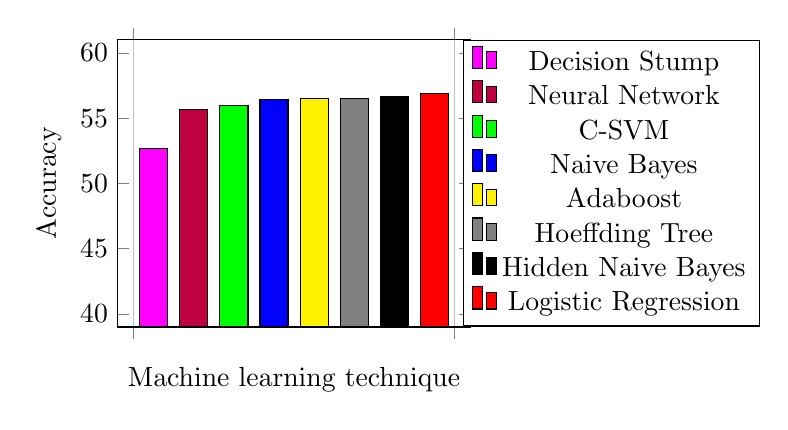
\begin{tikzpicture}
    \begin{axis}[
      %x tick label style={/pgf/number format/1000 sep=},
      xticklabel=\empty,
      ylabel=Accuracy,
      xlabel=Machine learning technique,
      enlargelimits=0.05,
      legend style={at={(1.4,1.0)},
        anchor=north,legend columns=1},
      ybar interval=0.7,
      width=.50\textwidth,
      ymin=40, ymax=60,
      reverse legend,
      ]
      \addplot[fill=red] coordinates {(1,56.916) 
        (0,2)
      };
      \addplot[fill=black] coordinates {(1,56.6807) 
        (0,56.6807)
      };

\addplot[fill=gray] coordinates {(1,56.48)
        (0,0)
      };      
            
      \addplot[fill=yellow] coordinates {(1,56.479) 
        (0,2)
      };
      \addplot[fill=blue] coordinates {(1,56.4454) 
        (0,56.4454)
      };
      \addplot[fill=green] coordinates {(1,55.98)
        (0,0)
      };
      \addplot[fill=purple] coordinates {(1,55.6555) 
        (0,0)
      };      
      \addplot[fill=Fuchsia] coordinates {(1,52.64)
        (0,0)
      };
      \legend{Logistic Regression,Hidden Naive Bayes,Hoeffding Tree,Adaboost,Naive Bayes,C-SVM,Neural Network, Decision Stump}
    \end{axis} 
  \end{tikzpicture}
  \caption{Test of best machine learning technique}\label{fig:besttech}
\end{figure}

The accuracies shown in \Cref{fig:besttech} were achieved after having adjusted the parameters of each method. The best parameters were found to be:
\begin{itemize}
\item C-SVM: sigmoid kernel function, $c = 1$.
\item Adaboost: 200 iterations
\item Logistic regression: L2-regularisation constant = 0.0016
\item Neural network: $(\text{attributes} + \text{classes}) / 2$ hidden neurons.
\item Hoeffding tree: Hoeffding tie threshold: 0.001, leaf prediction strategy: Naive bayes.
\end{itemize}

As seen in \Cref{fig:besttech}, most of the algorithms achieve an accuracy close to $56 \%$. Only the Decision Stump seems to be an outlier. However, this is expected, since the decision stump only bases its prediction on the value of one single feature.
Logistic Regression achieves the best accuracy. Since it also scaled well for parallel computation, we chose Logistic Regression for further tests.

\subsubsection{Feature symmetry experiment}
In \Cref{sec:representationoffeatures} we represented four different ways of representing features, to capture a possible symmetry in the choice of champions and the layout of the map. In this section we test each representation by training a classifier using logistic regression using the given representation of features. The experiment was performed on a test set of 10,000 matches with training sets of up to 50,000 matches. The result, shown in \Cref{fig:feat-rep}, indicates that binary and ternary are very close, but the mirrored is not far behind. The compact is the only representation that shows some weakness, this is because it is actually missing information, it does not contain the opposing team, which means it is missing a valuable connection. The binary representation seems slightly more accurate than the ternary in the majority of the time. Therefore we choose to conduct all the following tests using the binary representation. 

\begin{figure}[!htb]
  \centering
  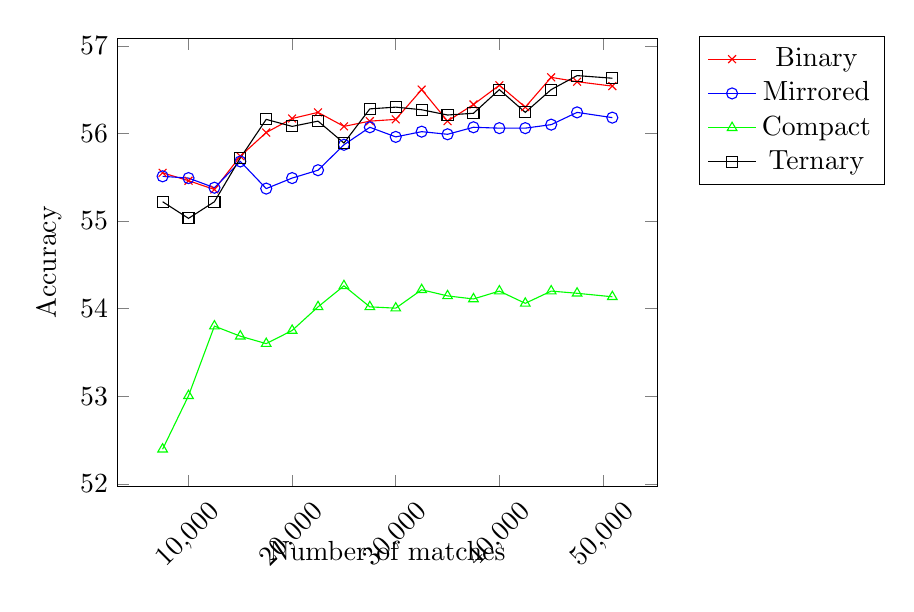
\begin{tikzpicture}[] 
    \begin{axis}[
      xlabel=Number of matches, 
      ylabel=Accuracy,
      xtick={10000,20000,30000,40000,50000},
      xticklabel style={rotate=45,anchor=near xticklabel},
      scaled x ticks=false,
      x label style={at={(axis description cs:0.5,-0.1)},anchor=north},
      legend style={at={(1.25,1.005)},
        anchor=north,legend columns=1},] 
      \addplot[color=red,mark=x] coordinates { 
        (7500, 55.55)
        (10000, 55.46)
        (12500, 55.36)
        (15000, 55.74)
        (17500, 56.01)
        (20000, 56.17)
        (22500, 56.24)
        (25000, 56.08)
        (27500, 56.14)
        (30000, 56.16)
        (32500, 56.50)
        (35000, 56.14)
        (37500, 56.33)
        (40000, 56.55)
        (42500, 56.30)
        (45000, 56.64)
        (47500, 56.59)
        (50901, 56.54)
      };
      \addplot[color=blue,mark=o] coordinates { 
        (7500, 55.51)  
        (10000, 55.49)
        (12500, 55.38)
        (15000, 55.68)
        (17500, 55.37)
        (20000, 55.49)
        (22500, 55.58)
        (25000, 55.87)
        (27500, 56.07)
        (30000, 55.96)
        (32500, 56.02)
        (35000, 55.99)
        (37500, 56.07)
        (40000, 56.06)
        (42500, 56.06)
        (45000, 56.10)
        (47500, 56.24)
        (50901, 56.18)
      };
      \addplot[color=green,mark=triangle] coordinates { 
        (7500, 52.395)  
        (10000, 53.005)
        (12500, 53.80)
        (15000, 53.685)
        (17500, 53.60)
        (20000, 53.75)
        (22500, 54.02)
        (25000, 54.26)
        (27500, 54.02)
        (30000, 54.005)
        (32500, 54.215)
        (35000, 54.145)
        (37500, 54.11)
        (40000, 54.20)
        (42500, 54.06)
        (45000, 54.20)
        (47500, 54.175)
        (50901, 54.135)
      };
      \addplot[color=black,mark=square] coordinates {
        (7500, 55.22)  
        (10000, 55.03)
        (12500, 55.22)
        (15000, 55.72)
        (17500, 56.16)
        (20000, 56.08)
        (22500, 56.14)
        (25000, 55.89)
        (27500, 56.28)
        (30000, 56.30)
        (32500, 56.27)
        (35000, 56.21)
        (37500, 56.23)        
        (40000, 56.50)
        (42500, 56.24)
        (45000, 56.50)
        (47500, 56.66)
        (50901, 56.63)
      };
      \legend{Binary, Mirrored, Compact, Ternary}
    \end{axis} 
  \end{tikzpicture}
  \caption{Test for representation of features}\label{fig:feat-rep}
\end{figure}

\subsubsection{Best features}
\label{sec:best-features}
To get an idea of each type of features impact on our prediction capability, some quick tests are performed using the machine learning tool Weka.
Logistic regression is used as classifier with an L2-regularisation parameter of 750 \todo{fik vi dobbelttjekket de 750?}. A training set of ranging size is used, up to a total of 50,000 matches, and a test set of 10,000 matches is used for evaluation \todo{forstår ikke denne sætning}. 
The obtained accuracies can be seen in \Cref{fig:best-feat}. Note that the $\phi_\text{CHAMPION-RUNE}$ feature type is not included, as it includes too many features for Weka to handle on a single machine with 8GB memory.
Interestingly, the baseline where no features are used gives an accuracy of $51.24 \%$, and results in a model that always predicts the blue team to win.
Note that the baseline is a flat line because it is clear already after 1,000 matches that the blue team wins the most, thus adding more training data does not change the learned model that always predicts the blue team to be the winner. Since the test set is the same regardless of how much training data that is used, the plot is a flat line. For the same reason, the $\phi_\text{BEST-RANKED}$ feature type also shows up as a straight line, because 1,000 matches is enough to learn a model that predicts the winning team to be the team with the highest average rank of its players.
Among the feature types that only consider the rank of players, the $\phi_\text{LANE-RANKS}$ feature did best.

When using more types of features at the same time, one may think that the accuracy always improves, but this is however not the case.
If all three types of features concerned with player ranks are used, an accuracy of only $56.06\%$ is achieved compared to $56.39\%$ when using the $\phi_\text{LANE-RANKS}$ features alone. There is no combination of rank feature types that gives a better accuracy than just using the best of them alone.
However, combining feature types that captures different phenomenons seems to increase the accuracy.
Among the tested feature types, the best feature types to combine has been found to be the $\phi_\text{LANE-RANKS}$ and $\phi_\text{LANE-CHAMPION}$ feature types from which an accuracy of $58.73 \%$ were achieved.

\begin{figure}[!htb]
  \centering
  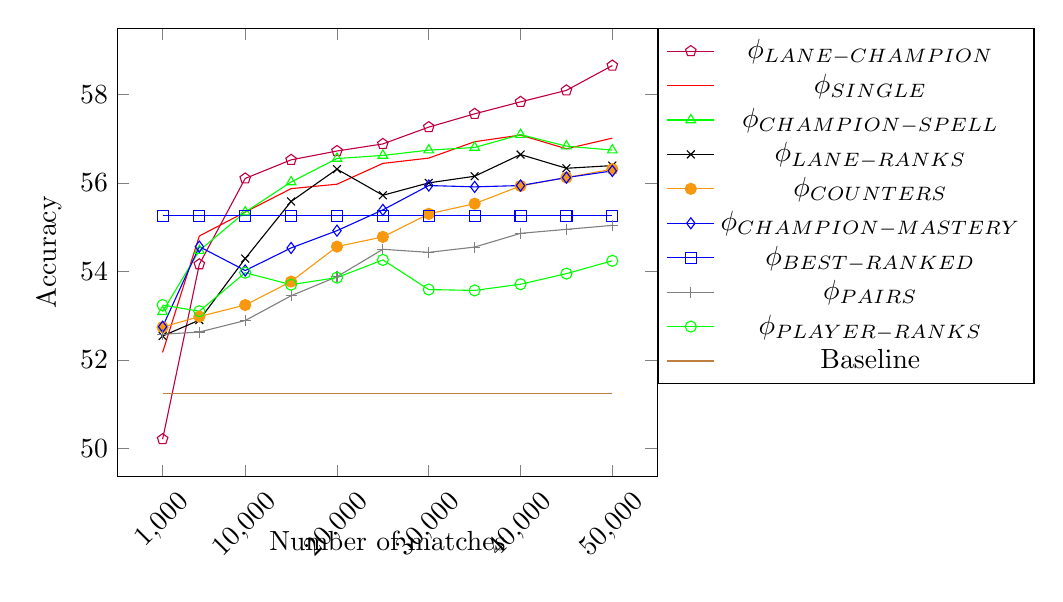
\begin{tikzpicture}[] 
    \begin{axis}[
      xlabel=Number of matches, 
      ylabel=Accuracy,
      xtick={1000,10000,20000,30000,40000,50000},
      xticklabel style={rotate=45,anchor=near xticklabel},
      scaled x ticks=false,
      x label style={at={(axis description cs:0.5,-0.1)},anchor=north},
      legend style={at={(1.35,1.001)},
        anchor=north,legend columns=1},] 
      \addplot[color=purple,mark=pentagon] coordinates { 
        (1000,50.21)
        (5000,54.16)
        (10000,56.10)
        (15000,56.52)
        (20000,56.72)
        (25000,56.88)
        (30000,57.26)
        (35000,57.56)
        (40000,57.83)
        (45000,58.09)
        (50000,58.65)
      };
       \addplot[color=red,mark=otime] coordinates { 
        (1000,52.17)
        (5000,54.8)
        (10000,55.34)
        (15000,55.87)
        (20000,55.97)
        (25000,56.44)
        (30000,56.56)
        (35000,56.93)
        (40000,57.08)
        (45000,56.77)
        (50000,57.01)
      };
      \addplot[color=green,mark=triangle] coordinates { 
        (1000,53.09)
        (5000,54.47)
        (10000,55.34)
        (15000,56.02)
        (20000,56.55)
        (25000,56.62)
        (30000,56.74)
        (35000,56.8)
        (40000,57.09)
        (45000,56.83)
        (50000,56.74)
      };
      \addplot[color=black,mark=x] coordinates { 
        (1000,52.54)
        (5000,52.90)
        (10000,54.29)
        (15000,55.58)
        (20000,56.31)
        (25000,55.72)
        (30000,56.00)
        (35000,56.15)
        (40000,56.64)
        (45000,56.33)
        (50000,56.39)
      };
      \addplot[color=YellowOrange,mark=*] coordinates { 
        (1000,52.74)
        (5000,52.98)
        (10000,53.24)
        (15000,53.77)
        (20000,54.56)
        (25000,54.78)
        (30000,55.3)
        (35000,55.53)
        (40000,55.93)
        (45000,56.12)
        (50000,56.31)
      };
      \addplot[color=blue,mark=diamond] coordinates { 
        (1000,52.75)
        (5000,54.56)
        (10000,54.02)
        (15000,54.53)
        (20000,54.92)
        (25000,55.39)
        (30000,55.94)
        (35000,55.91)
        (40000,55.94)
        (45000,56.12)
        (50000,56.27)
      };
      \addplot[color=blue,mark=square] coordinates { 
        (1000,55.26)
        (5000,55.26)
        (10000,55.26)
        (15000,55.26)
        (20000,55.26)
        (25000,55.26)
        (30000,55.26)
        (35000,55.26)
        (40000,55.26)
        (45000,55.26)
        (50000,55.26)
      };
      \addplot[color=gray,mark=+] coordinates { 
        (1000,52.58)
        (5000,52.63)
        (10000,52.89)
        (15000,53.45)
        (20000,53.88)
        (25000,54.5)
        (30000,54.43)
        (35000,54.55)
        (40000,54.86)
        (45000,54.95)
        (50000,55.04)
      };
       \addplot[color=green,mark=o] coordinates { 
        (1000,53.24)
        (5000,53.1)
        (10000,53.97)
        (15000,53.7)
        (20000,53.86)
        (25000,54.26)
        (30000,53.59)
        (35000,53.57)
        (40000,53.71)
        (45000,53.95)
        (50000,54.24)
      };
      \addplot[color=brown] coordinates { 
        (1000,51.24)
        (5000,51.24)
        (10000,51.24)
        (15000,51.24)
        (20000,51.24)
        (25000,51.24)
        (30000,51.24)
        (35000,51.24)
        (40000,51.24)
        (45000,51.24)
        (50000,51.24)
      };

\legend{$\phi_\text{LANE-CHAMPION}$,$\phi_\text{SINGLE}$,$\phi_\text{CHAMPION-SPELL}$,$\phi_\text{LANE-RANKS}$,$\phi_\text{COUNTERS}$,$\phi_\text{CHAMPION-MASTERY}$,$\phi_\text{BEST-RANKED}$,$\phi_\text{PAIRS}$,$\phi_\text{PLAYER-RANKS}$,Baseline}
     
    \end{axis} 
  \end{tikzpicture}
  \caption{Accuracy of features}\label{fig:best-feat}
\end{figure}


%%% Local Variables:
%%% mode: latex
%%% TeX-master: "../main"
%%% End:
